%************************************************
\chapter{Kubernetes}\label{ch:kubernetes}
%************************************************
In this chapter the Kubernetes cluster/container manager is briefly introduced. Furthermore, a proof-of-concept is made for Kubernetes running the different services from the Fruitshop. In the proof-of-concept following is done:
\begin{itemize}
	\item  All containerized services are deployed in Kubernetes on the Raspberry Pi cluster 
	\item Pods in Kubernetes are scaled 
	\item Pods are updated with \emph{rolling-update} 
\end{itemize}

\textbf{What is Kubernetes?}\\
Kubernetes is a cluster management tool made by google to manage containerized applications. Kubernetes takes a bunch of nodes and make them appear as a one big computer and deploy container applications to the public or private cloud based on preference. Kubernetes abstracts away the discrete nodes and optimizes compute resources.  

Moreover, Kubernetes make use of a declarative approach to get the desired state for the application mentioned by the user. 

Whenever an application is deployed onto the cluster, the Kubernetes' master node have to decide and deploy the application to the correct host. Kubernetes does all the heavy lifting by using its scheduler. 

Furthermore, Kubernetes is used for automating management of containers such as scaling, loadbalancing and scheduling containers between nodes in a cluster. Kubernetes makes the cluster environment much more robust for container deployment.

Containers in Kubernetes are run inside pods. A pod can contain a single or a group of containers which are scheduled onto the same host. They are used to gather containers that are tightly coupled to each other under the same host such that communication between containers becomes easier. Every pod has it's own ip address. Kubernetes schedules, deploy and scale pods such they among other ensure that the load is balanced in the cluster. 

The containers or the pods in the nodes can be replicated, so if one node fails Kubernetes will create a new pod on another node and run the container within this newly created pod. The Kubernetes keeps track of all the living pods using its built-in registry service.  
If there suddenly comes a lot of load on a specific node it will make extra \emph{replicaset} of the pods so that the load is distributed between these pods and thereby the load is more balanced but only if the Kubernetes is set to autoscale.\cite{bernstein2014containers}

\section{PoC of Kubernetes}
%Before running the containerized services within Kubernetes the verifying process was to run them on the local machine. As the services was behaving as intended on the local machine, it was verified that they were ready for beeing deployed as Docker containers inside Kubernetes on the cluster. 

%For running these services as Docker containers on the cluster it is necessary to put the service inside a Docker container from the cluster instead of locally.

%To deploy the service to Kubernetes its essential to build jar file within the cluster to have the rightful configuration setup.

%In the following step the Dockerfile is run on the cluster which puts the service inside a Docker container. When the service is packed within Docker container the service is then pushed to Docker hub.   

The first thing that is done for deploying the containerized services in Kubernetes on the Raspberry Pi cluster is to create a  yaml-file with the deployment configuration. The yaml-file for \eg the contact service image is created with help of the following command. 
\begin{lstlisting}[frame=single, ]
kubectl run contact --image=bilalkais/contact -l visualize=true,run=contact --dry-run --output=yaml > contact-deployment.yaml
\end{lstlisting}
Note: If the Docker image is not available in the cluster, it will be cloned from the Docker Hub repository.\\

The deployment of the contact service image can then be created with help of the newly generated yaml-file by use of the following command.
\begin{lstlisting}[frame=single, ]
kubectl create -f contact-deployment.yaml
\end{lstlisting}

To execute the contact service on the newly created pod, a yaml-file is created with the configuration of correct execution of the service, following command is used:
\begin{lstlisting}[frame=single, ]
kubectl expose deployment contact --port=9002 --target-port=9002 --external-ip=192.168.1.11 -l visualize="true",run=contact --dry-run --output=yaml > contact-svc.yaml
\end{lstlisting}

Then the contact service is executed with help of the generated yaml-file in the following command.
\begin{lstlisting}[frame=single, ]
kubectl create -f contact-svc.yaml
\end{lstlisting}

The config server is a good example of a service which has to be fault-tolerant as all the other services are depending on it to be able to load the configuration. It was chosen to scale the config server deployment to four replicas as shown in figure \ref{fig:configserver-visual}. 
\begin{figure}[bth]
	\centering 
	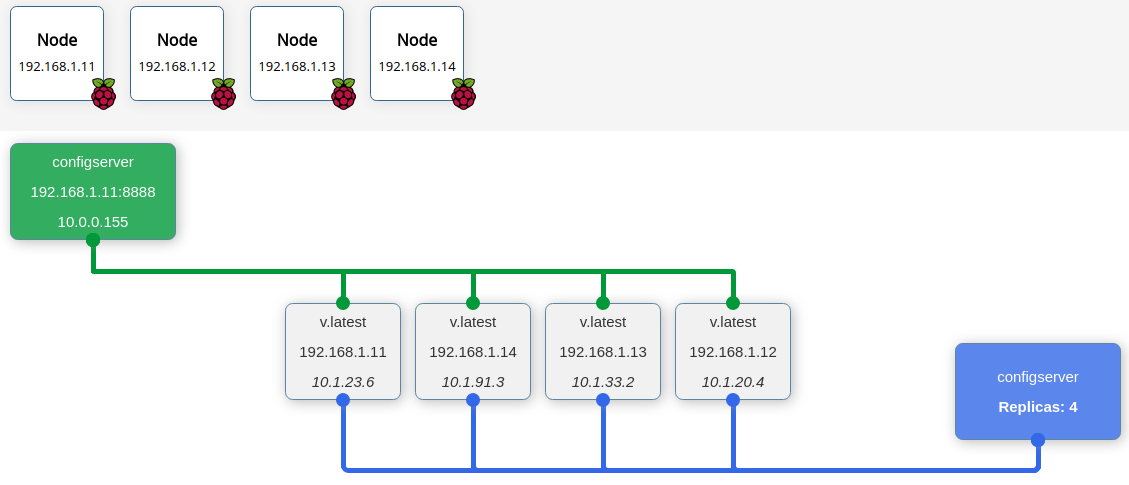
\includegraphics[width=1\linewidth]{gfx/configServer4Replicas}
	\caption[configserver]{Visualisation of Config Server replicas running in Kubernetes} \label{fig:configserver-visual}
\end{figure}
Following is the command used for scaling the deployment:
\begin{lstlisting}[frame=single, ]
kubectl scale deployment configserver --replicas=4
\end{lstlisting}

%Lastly we update the pods, using rolling-update:
%results image